\chapter{Jobs and Income}

\section*{Number of people supported to have raised incomes and better jobs  or livelihoods}

% make sure numbers and header don't appear
\thispagestyle{empty}


\section{Results}
From 2015/16 to 2019/20 DFID supported \textbf{5.1 million} people to raise their incomes or maintain/gain a better job or livelihood. %

\subsection{Results by gender}
Ninety-nine percent of results were broken down by gender. %
Of the 5.1 million people supported, 3.6 million were men and 1.5 million were women (figures do not sum due to rounding).

\subsection{Results by region}
See Figure \ref{fig:jobs_region_plot} for regional breakdown of results.  %


\begin{figure}[htbp]
	\centering
	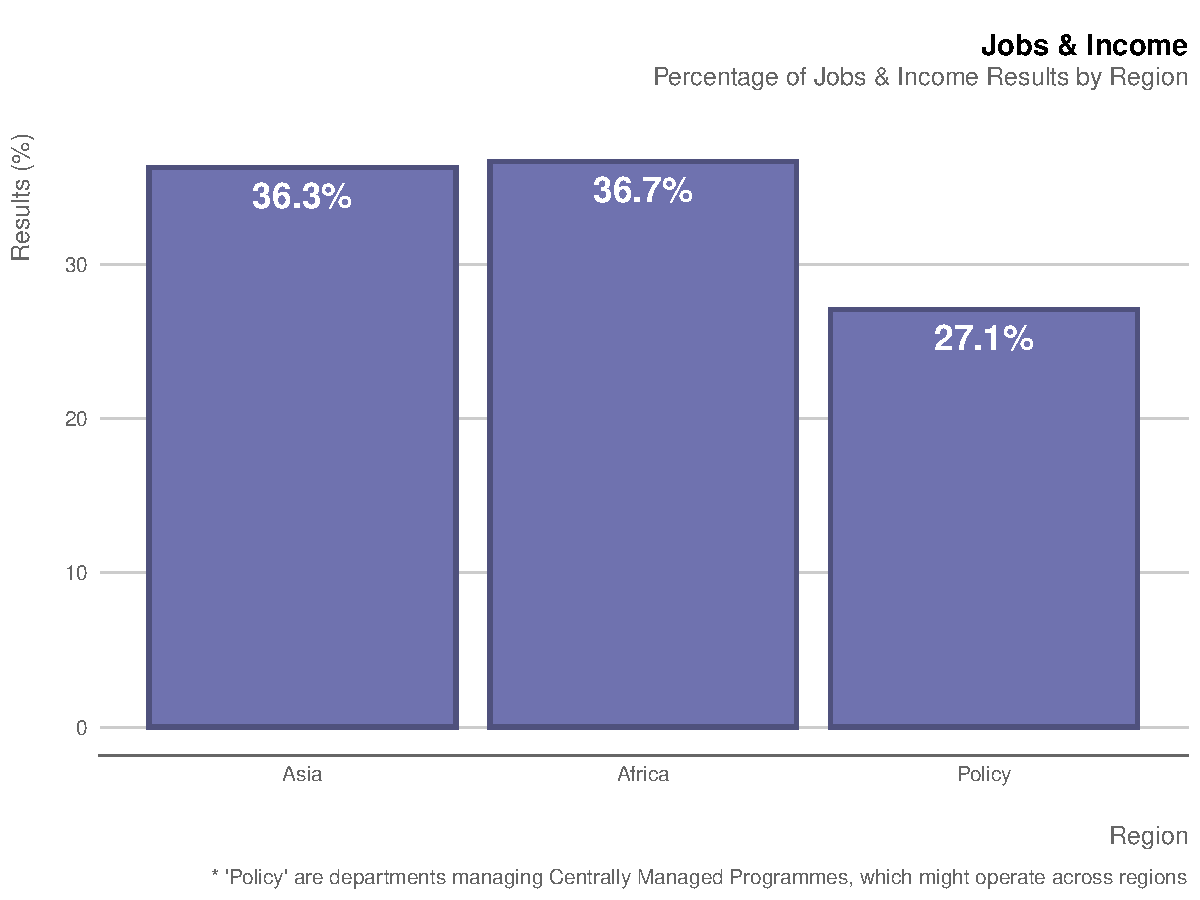
\includegraphics[width=0.8\textwidth]{../figs/jobs_region_plot} \hfill
	\caption{Percentage of Jobs and Income results by region.}
	\label{fig:jobs_region_plot}
\end{figure}



\subsection{Results by type}
Of the total 5.1 million people supported to raise their incomes or maintain/gain a better job or livelihood:

\begin{itemize}
\item 2.4 million people were supported to raise their income.
\item 1.9 million people were supported to gain or maintain a better job or livelihood. %
This includes figures for programmes which measured the number of jobs created/maintained, rather than have indicators which directly measure beneficiary numbers. %
However, a single beneficiary is assumed for every job maintained/created. %
\item The remaining 0.7 million people were beneficiaries for programmes where the indicator measured the total of all or some of the following:
	\begin{itemize}
		\item maintained income
		\item increased income
		\item maintained employment
		\item gained employment
		\item jobs created
		\item jobs supported
	\end{itemize}
\end{itemize}

Changes in the total number of people supported from previous years is affected by the composition of programmes reporting, as well as by new results from previously reporting programmes. %
Each year, new programmes may start reporting results eligible for inclusion in this indicator.  %

One significant change affecting results this year, is that we have included CDC results for the first time. %
CDC accounted for 0.85 million people supported\footnote{CDC numbers are in full-time equivalents, as per the HIPSO definition, and so are underestimates of individual beneficiaries eg seasonal and part time workers} (of which 28\% were Female and 72\% Male). %
Only beneficiary figures for 2018 (not for every year) have been included for CDC in the 2015/16 to 2019/20 DFID results. %
This is to avoid double counting the same beneficiaries who may otherwise appear in figures for multiple years. %
Note that CDC also reports indirect employment beneficiaries in supply chains, induced from wages, and enabled by productivity improvements from credit and power, estimated from the Joint Impact Model, which are not included in DFID’s aggregate figures.%


\section{Context}

DFID's overarching priority in economic development is to promote growth that creates more and better\footnote{Better jobs imply higher productivity and earnings, better benefits, better working conditions, and/or improved income protection, for example.} productive jobs and livelihoods to help people lift themselves out of poverty. %
Enhanced employment opportunities and skills is also a means to address the underlying drivers of instability and can support longer term security and stability. %

Results have been collected from 30 programmes across DFID. %T
These programmes all:
\begin{adjustwidth}{0.5cm}{}
Focused on job rich activities with an objective to either increase beneficiaries’ income from economic activity or get beneficiaries into more productive and/or better quality employment, and can provide a clear rationale of why and how the programme is doing this.
\end{adjustwidth}

\begin{adjustwidth}{8cm}{}
\textbf{AND}
\end{adjustwidth}

\begin{adjustwidth}{0.5cm}{}
The relevant jobs/income related effects on beneficiaries are monitored at least twice within the lifetime of the programme (e.g. within the logframe or regular surveys) within the existing monitoring.
\end{adjustwidth}

The exact definition of jobs/incomes is not stipulated for inclusion for this indicator as this will legitimately vary across countries, sectors and over time. %
In addition, the most suitable job/income indicator for programme monitoring will need to be programme-specific to maximise its value for monitoring. %
Following good monitoring practices, we expect indicators to be aligned with programme objectives. %

\newpage
